\documentclass{article}
\usepackage[papersize={7in,5in}, top=1in, bottom=0in, left=1in, right=1in]{geometry}
\usepackage{tikz}
\usepackage[default]{sourcesanspro}
\usepackage[T1]{fontenc}

\pagenumbering{gobble}

\newenvironment{sentencediagram}[3]
    {
        \begin{center}
            {
                \fontfamily{cmr}\selectfont
                #1 \newline
            }

            \footnotesize #2, \textit{#3}
            \vspace{0.5cm}
            \Large 
    }
    {\end{center}}

\definecolor{subjectnoun}{RGB}{106,120,132}
\definecolor{copula}{RGB}{124,139,111}
\definecolor{subjectcomplement}{RGB}{77,47,13}
\definecolor{conjunction}{RGB}{56,84,129}
\definecolor{preposition}{RGB}{32,129,159}
\definecolor{directobject}{RGB}{231,51,143}
\definecolor{adjective}{RGB}{103,81,120}
\definecolor{noun}{RGB}{190,103,93}
\definecolor{predicateverb}{RGB}{176,161,118}
\definecolor{article}{RGB}{62,23,85}

\begin{document}
    \begin{sentencediagram}{It was a bright cold day in April, and the clocks were striking thirteen.}{George Orwell}{1984}
        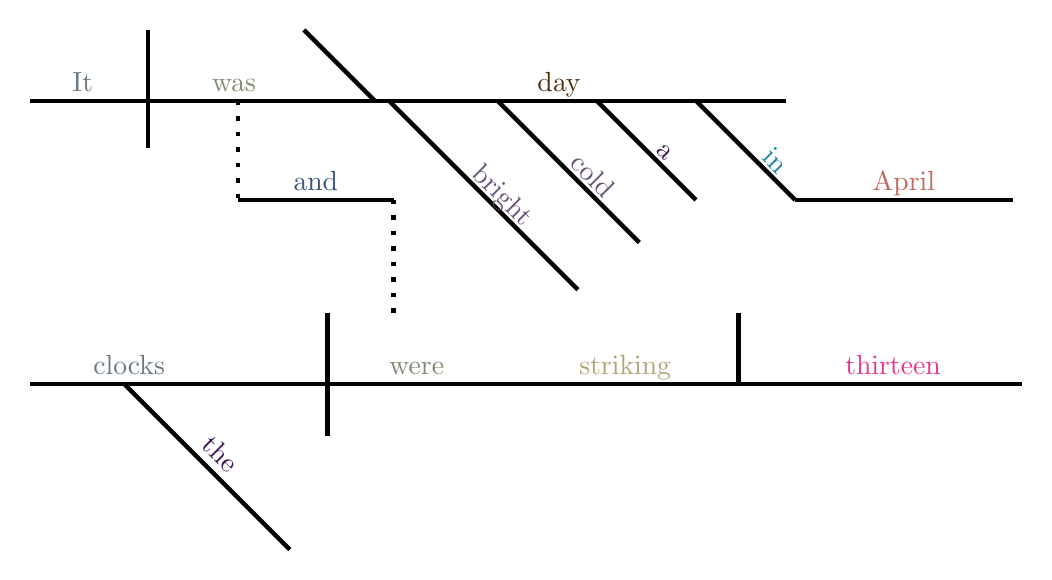
\begin{tikzpicture}[scale=1.2]
            \tikzstyle{every node} = [above=-0.15cm]
            \draw[ultra thick] (-5, 1.75) -- (3, 1.75)
                node[pos=.07, text=subjectnoun]{\strut It}
                node[pos=.27, text=copula]{\strut was}
                node[pos=.7, text=subjectcomplement]{\strut day};
            \draw[ultra thick] (-3.75, 2.5) -- (-3.75, 1.25);
            \draw[ultra thick] (-2.1, 2.5) -- (-1.35, 1.75);
            \draw[ultra thick] (-1.2, 1.75) -- (0.8, -0.25)
                node[above=-0.06cm, sloped, pos=0.55, text=adjective]{\strut bright};
            \draw[ultra thick] (-0.05, 1.75) -- (1.45, 0.25)
                node[above=-0.06cm, sloped, pos=0.6, text=adjective]{\strut cold};
            \draw[ultra thick] (1, 1.75) -- (2.05, 0.7)
                node[above=-0.06cm, sloped, pos=0.6, text=article]{\strut a};
            \draw[ultra thick] (2.05, 1.75) -- (3.1, 0.7)
                node[above=-0.06cm, sloped, pos=0.7, text=preposition]{\strut in};

            \draw[loosely dotted, ultra thick] (-2.8, 1.75) -- (-2.8, 0.7);
            \draw[ultra thick] (-2.8, 0.7) -- (-1.15, 0.7)
                node[pos=.5, text=conjunction]{\strut and};
            \draw[ultra thick] (3.1, 0.7) -- (5.4, 0.7)
                node[pos=.5, text=noun]{\strut April};
            \draw[loosely dotted, ultra thick] (-1.15, 0.7) -- (-1.15, -0.5);

            \draw[ultra thick] (-5, -1.25) -- (5.5, -1.25)
                node[pos=.1, text=subjectnoun]{\strut clocks}
                node[pos=.39, text=copula]{\strut were}
                node[pos=.6, text=predicateverb]{\strut striking}
                node[pos=.87, text=directobject]{\strut thirteen};
            \draw[ultra thick] (-1.85, -0.5) -- (-1.85, -1.8);
            \draw[ultra thick] (2.5, -1.25) -- (2.5, -0.5);
            \draw[ultra thick] (-4, -1.25) -- (-2.25, -3.0)
                node[sloped, pos=.5, text=article]{\strut the};
        \end{tikzpicture}
    \end{sentencediagram}
    
    \begin{sentencediagram}{All of this happened, more or less.}{Kurt Vonnegut}{Slaughterhouse Five}
        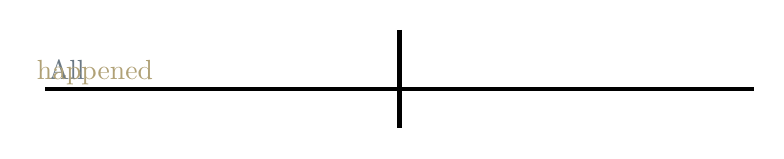
\begin{tikzpicture}
            \tikzstyle{every node} = [above=-0.15cm]
            \draw[ultra thick] (-5, 2) -- (4, 2)
                node[pos=.03, text=subjectnoun]{\strut All}
                node[pos=.07, text=predicateverb]{\strut happened};
            \draw[ultra thick] (-0.5, 2.75) -- (-0.5, 1.5);
        \end{tikzpicture}
    \end{sentencediagram}
\end{document}
